\documentclass[12pt,a4paper]{scrartcl}
    \usepackage[utf8]{inputenc}
    \usepackage{amsmath}
    \usepackage{amsfonts}
    \usepackage{amssymb}
    \usepackage{graphicx}
\usepackage{array,booktabs,calc}

    \usepackage[bottom = 1in, left = 0.5in, right = 0.5in, top = 1in]{geometry}

    \usepackage[english]{babel}
    \usepackage[autostyle]{csquotes}
    \usepackage{mathptmx}

    \usepackage[labelfont=bf]{caption}

    \usepackage[default, scale=0.95]{opensans}

    \usepackage[T1]{fontenc}

	\usepackage{fixltx2e}
	
	\usepackage{textcomp}

    %\addto\captionsenglish{\renewcommand{\figurename}{Fig.}}
    % \addto\captionsenglish{\renewcommand{\tablename}{Supplementary Table}}
	
	
	
	%\captionsetup[figure]{labelfont={bf},name={Fig. A},labelsep=period, labelsep=none}

	\title{Supplementary material}
	\date{}
	
\begin{document}
\maketitle

\section*{Appendix A}

\renewcommand{\thefigure}{A\arabic{figure}}%
\renewcommand{\thetable}{A\arabic{table}}
\setcounter{figure}{0}
\setcounter{table}{0}

\begin{figure}[h]
	\centering
	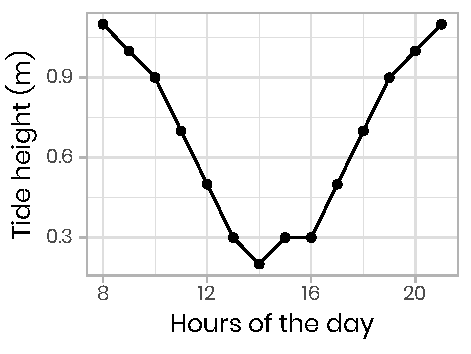
\includegraphics[scale = 1]{../../../graphs/supp_fig01.pdf}
	\caption{Surface tidal height versus time at Qikiqtarjuaq measured on 2015-06-09.}
\end{figure}

\clearpage
\newpage

\section*{Appendix B}

\renewcommand{\thefigure}{B\arabic{figure}}%
\renewcommand{\thetable}{B\arabic{table}}
\setcounter{figure}{0}
\setcounter{table}{0}

\begin{figure}[h]
	\centering
	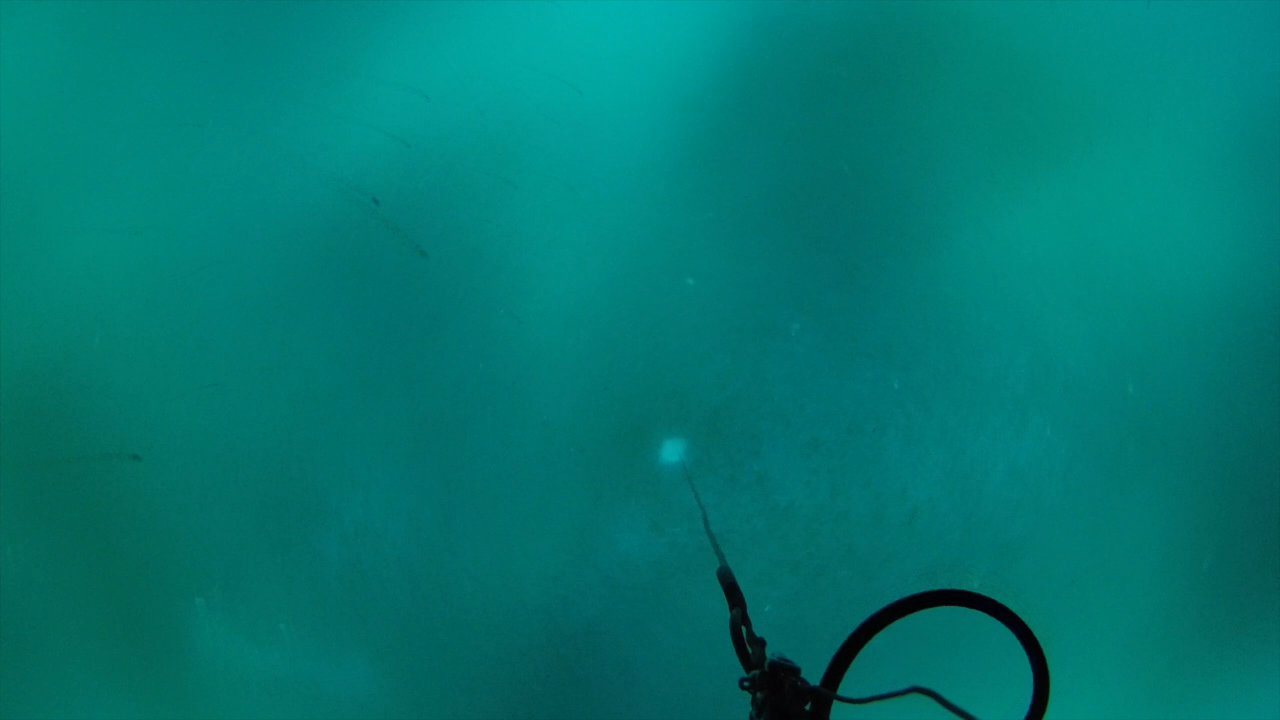
\includegraphics[scale = 0.35]{../../../gopro_images/Frame_720P_at_00_58_LowSnow_20150518.png}
	\caption{Video frame (00:58) from GoPro Hero 4 recording of C-OPS descent from 0 to 30 m, 18 May 2015 at the "low snow" hole. Note the streaks of nekton swimming across the upper left quadrant of the frame. Many planktons were seen in this profile, indicating an active under-ice community. A profile of the "high snow" hole on the same day, just 40 m away, showed no such plankton activity.}
\end{figure}

\clearpage
\newpage

\begin{center}
	\captionof{table}{Example GoPro Hero 4 photos at the low and high snow holes in 2015 demonstrate the spatial variability of the ice bottom across time and space.}
	\begin{tabular}{| m{.1\textwidth} | m{.25\textwidth} | m{.25\textwidth} | m{.25\textwidth} |}
		\hline
		\textbf{} & \textbf{18 May 2015}                                                                              & \textbf{31 May 2015}                                                                              & \textbf{12 June 2015}                                                                             \\
		\hline
		Low~snow  & 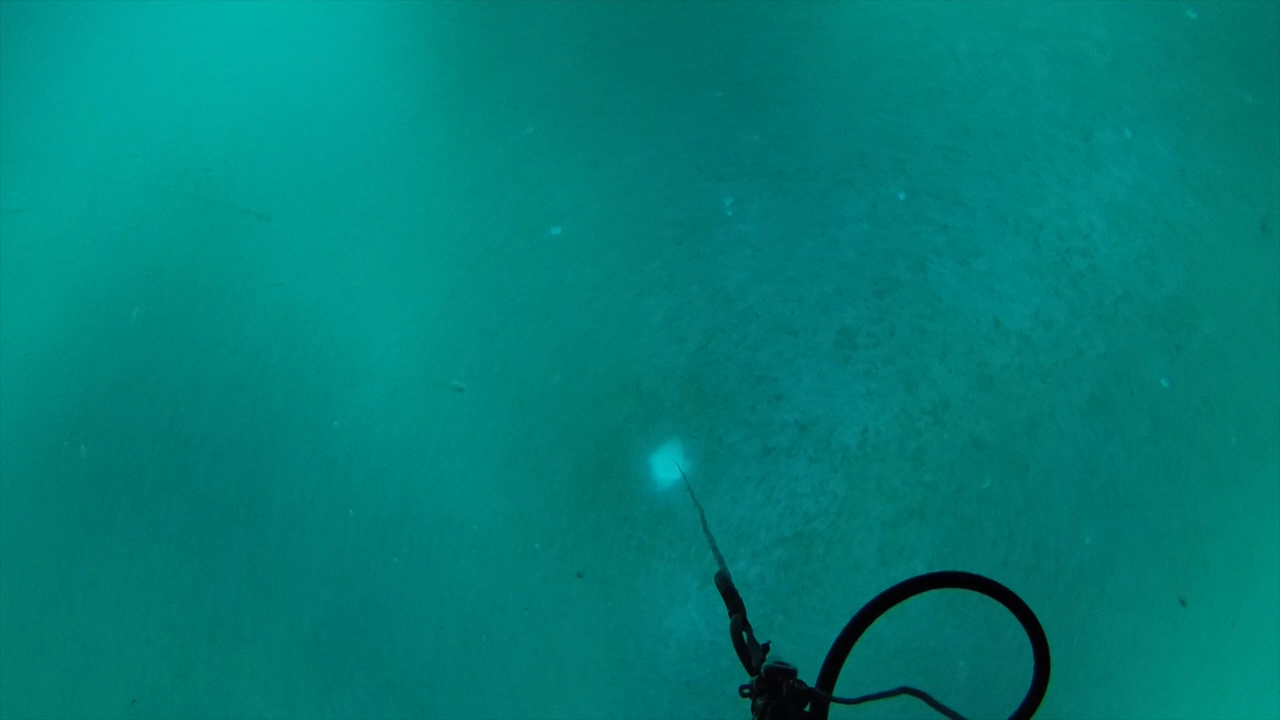
\includegraphics[scale=0.1] {../../../gopro_images/Frame_1_1_720P_at_00_43_LowSnow_20150518.png}  & 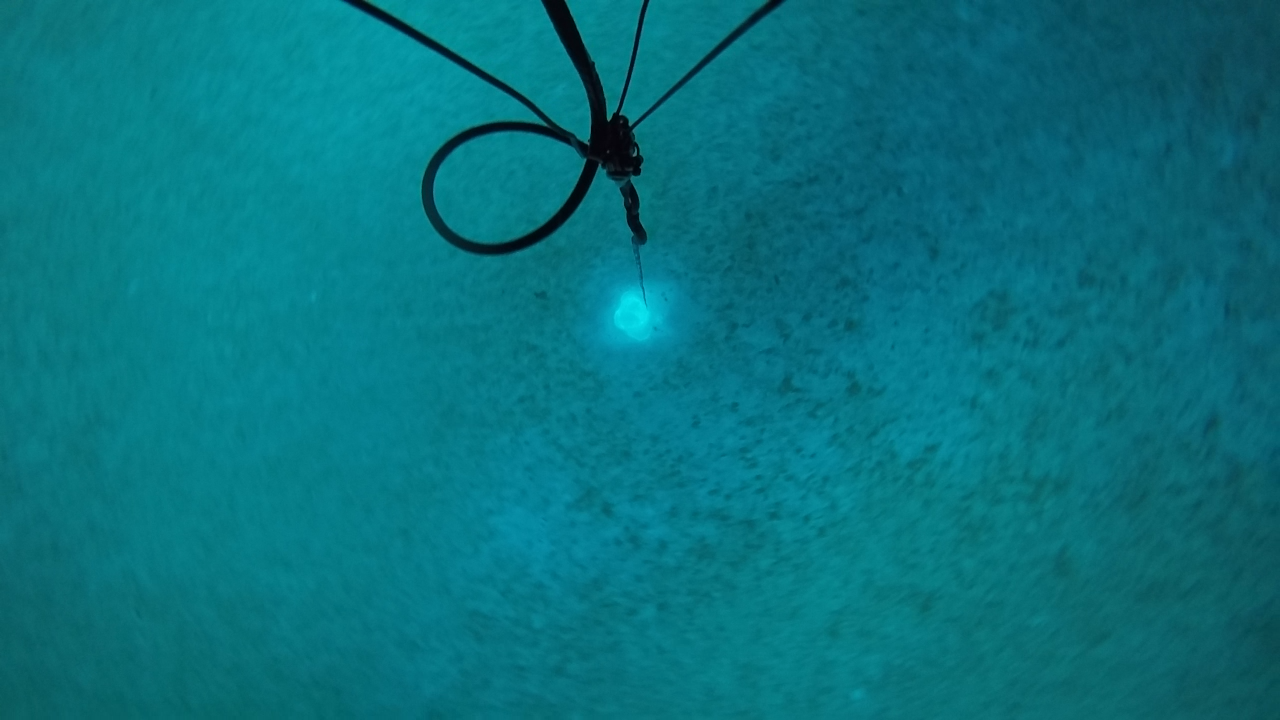
\includegraphics[scale=0.1] {../../../gopro_images/Frame_1_2_720P_at_06_02_LowSnow_20150531.png}  & 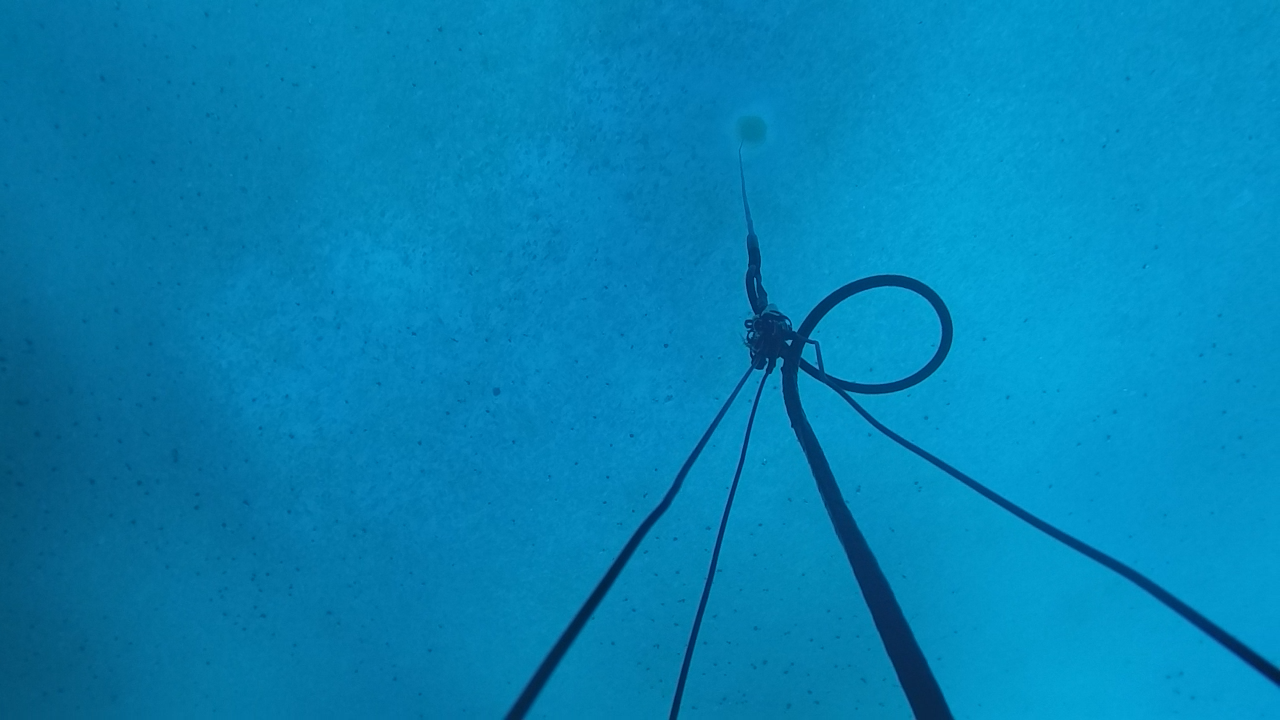
\includegraphics[scale=0.1] {../../../gopro_images/Frame_1_3_720P_at_06_37_LowSnow_20150612.png}  \\
		\hline
		High~snow & 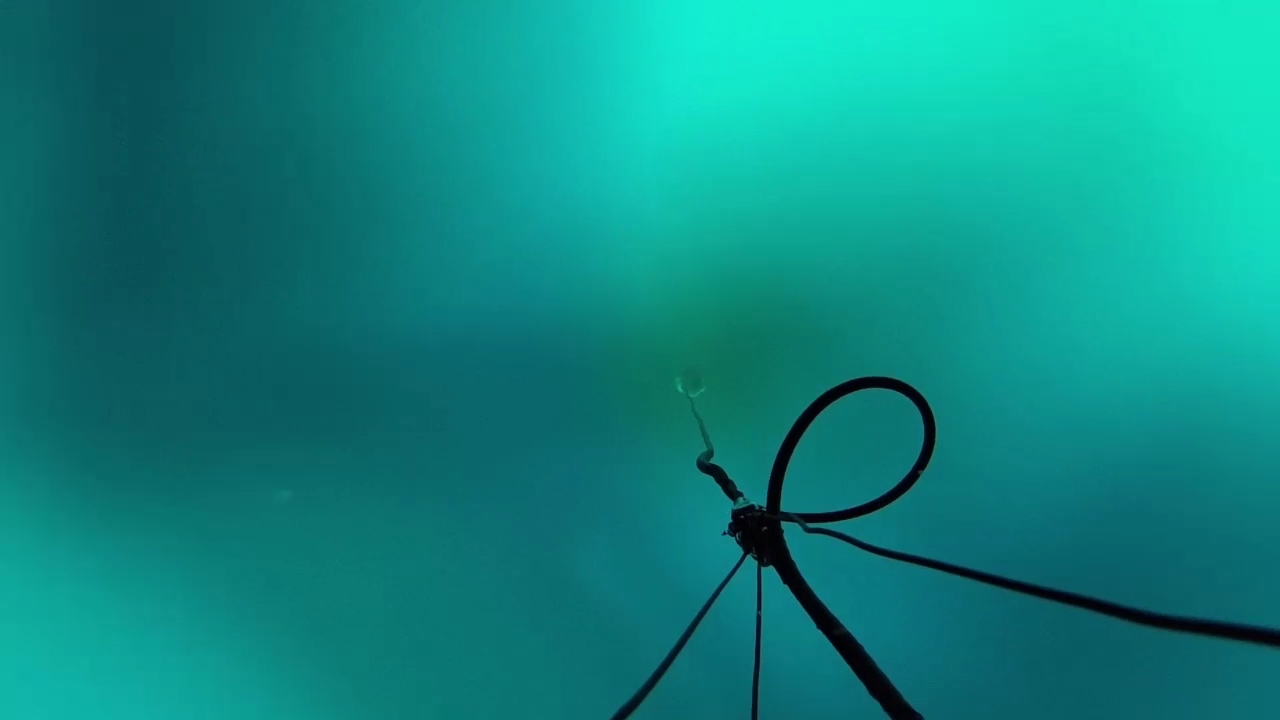
\includegraphics[scale=0.1] {../../../gopro_images/Frame_2_1_720P_at_00_50_HighSnow_20150518.png} & 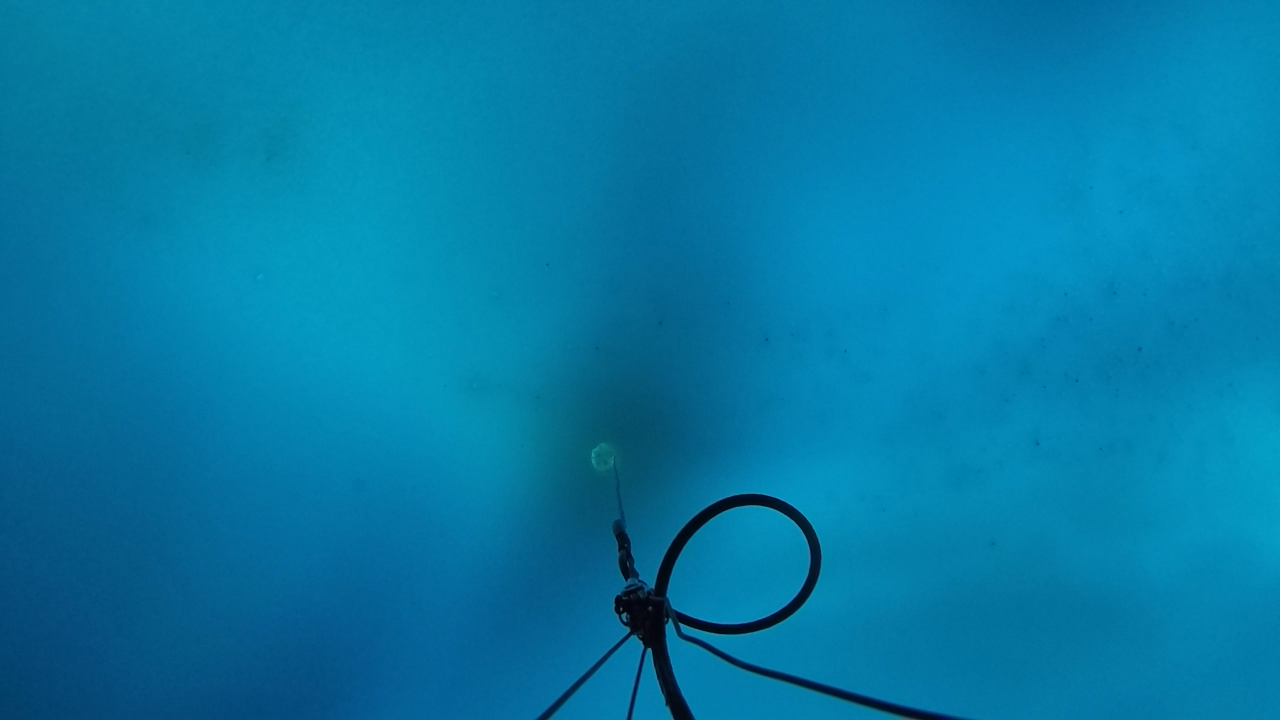
\includegraphics[scale=0.1] {../../../gopro_images/Frame_2_2_720P_at_05_15_HighSnow_20150531.png} & 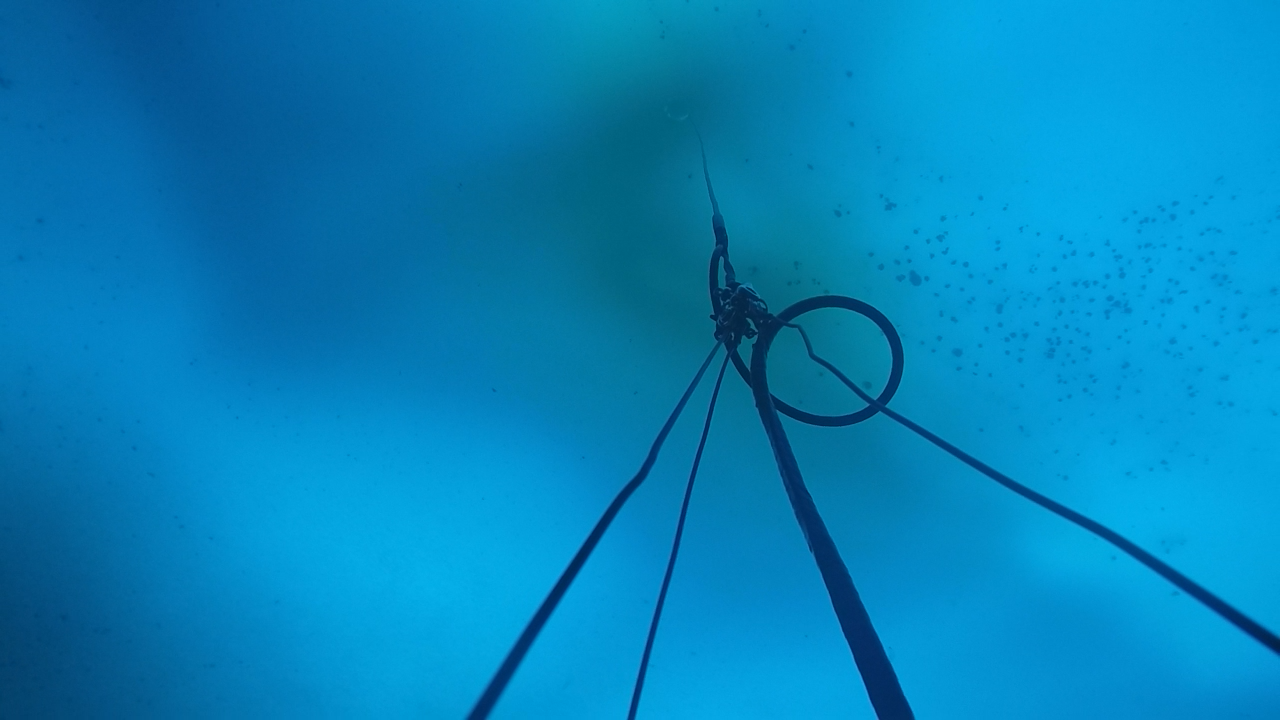
\includegraphics[scale=0.1] {../../../gopro_images/Frame_2_3_720P_at_11_20_HighSnow_20150612.png} \\
		\hline
	\end{tabular}

\end{center}




\end{document}
